\documentclass[letterpaper]{article}


\PassOptionsToPackage{numbers}{natbib}
\usepackage[preprint]{neurips_2023}
\usepackage[utf8]{inputenc} % allow utf-8 input
\usepackage[T1]{fontenc}    % use 8-bit T1 fonts
\usepackage{hyperref}       % hyperlinks
\usepackage{url}            % simple URL typesetting
\usepackage{booktabs}       % professional-quality tables
\usepackage{amsfonts}       % blackboard math symbols
\usepackage{nicefrac}       % compact symbols for 1/2, etc.
\usepackage{microtype}      % microtypography
\usepackage{xcolor}         % colors
\usepackage{tikz}
\usepackage{pgfplots}
\usepackage{tabularx,ragged2e}


\newcolumntype{L}{>{\RaggedRight}X}
\pgfplotsset{width=10cm,compat=1.9}


%%%%%%%%%%%%%%%%%%%%%%%%%%%%%%%%%%%%%%%%%%%%%%%%%%%%%%%%%%%%


\title{GNN as Policy Network for Deep Reinforcement Learning Generalization}

\author{%
    Roozmehr Jalilian, Shidi Xi \\
    Department of Electrical \& Computer Engineering \\
    The University of British Columbia \\
    \texttt{\{roozmehr.jalilian,xsd99\}@ece.ubc.ca} \\
    Vancouver, BC V6T 1Z4
}


\begin{document}


\maketitle


\begin{abstract}
Routing, which can be modeled as a pathfinding problem,  has always been one of the most challenging stages of integrated circuits (IC) design, both in terms of complexity and time consumption. Even with state-of-the-art commercial CAD tools, complex designs can take hours and maybe days to be routed. Thus, there has been a surge of interest to use machine-learning-based approaches to tackle these difficulties. In a previous work, we have proposed a novel reinforcement learning (RL) approach for routing. Although the RL router can deliver better solutions than a baseline, it suffers from poor generalizability, that is, every problem has to be solved by training a policy from scratched. Hence, in this work, we propose a novel graph neural network (GNN) and implement it as the policy network of the RL router. This enables the agents to generalize their learned routing strategy to new, unseen designs and saves computation time.
\end{abstract}

\section{Introduction}
IC routing is the process of connecting different electrical contact points (pins) on a chip with metallic wires. For example, the CPU and the memory in a computer chip must be connected with wires such that they can transfer data and do computing. We can model routing as a pathfinding problem, where the chip is abstracted into a 2-dimensional grid, and the pins, defined by (x, y) coordinates, sit on the nodes of this grid. The task is then to find paths between the specified nodes by traversing through the grid edges. In addition, each edge has a feature called the capacity, which represents the maximum number of wires permitted to use this edge. This constraint comes from the fact that in a real physical world, each wire has some thickness, and the number of wires allowed within a chip region is finite. If the usage of an edge exceeds its capacity, the edge is overflowed, which is highly undesirable. Hence, to find a optimal routing solution, we need to determine optimal paths to connect pins to minimize the total wirelength while maintaining zero edge overflow.

A set of pins that need to be connected together is called a net, and during a routing process, there will be many nets that must be routed, they form a set called the netlist. For the rest of this proposal, we will use the term nodes interchangiablly with pins.

In our previous work, we proposed an multi-agent RL router to solve the IC routing problem, where each agent is responsible for routing one net, and they take actions concurrently. We designed the agents to be homogeneous and fully-cooperative, and hence, they are governed by one super policy. The RL router was trained using proximal policy optimization (PPO) (REF), and was evaluated using benchmarks. The results showed the RL router can significantly outperform an A* baseline, however, the policy trained for one benchmark does not generalize to other unseen although very similar problems. After extensive analysis, we conclude the reason is because the policy neural network, consists of several full-connected (FC) layer, cannot learn rich information from the state encodings and thus has poor generalizability.

As opposed to a multi-layer perceptron (MLP), GNNs can generalize well when dealing with graphical data (REF), which is the case for routing problem that can be modeled as a grid graph. Therefore, in this project we propose a novel message-passing GNN architecture, which will be embedded into our developed RL router as the policy network. The GNN will take the routing grid graph from the environment as the state input and output actions. The aim is to enhance the router, such that it can generalize trained policies to unseen but similar problems, and hence, achieve significant improvement in terms of computation time.

 

%Digital logic design involves three major stages: {\bf RTL}\footnote{Register transfer level}{\bf design}, {\bf synthesis}, and {\bf physical design}. An engineer first decides on the architecture of a digital circuit, and describes it with the help of a {\it hardware description language} (HDL). The described architecture is then fed into a CAD tool, which first synthesizes the design using different logic gates, and then maps the gates onto the chip canvas.

%Physical design is perhaps the most challenging stage of the whole process, as it involves two sophisticated and time-consuming phases: {\bf placement} and {\bf routing}. The goal of this stage is to place a large number of logic gates on the chip and route them in such a way that the final circuit satisfies multiple constraints (timing, area, etc.). Routing, in general, is the more complex, as the wiring resources on the chip are limited and routing {\bf congestion} must also be taken into account.

%Due to the problem's complexity, routing is generally broken into two sub-phases: {\bf global} and {\bf detailed}. Global routing first partitions the chip into routing regions and searches for region-to-region paths for all signal nets; this is followed by detailed routing, which determines the exact tracks and vias of these nets based on their region assignments \cite{Kahng2022}.

%Obtaining a valid solution which satisfies all constraints might usually take up to several days for large circuits, leading to a surge of interest to use machine learning techniques, aiming to find solutions much faster while improving or maintaining the same level of solution quality.

%TODO: RL approach, poor generalizability, propose GNN as policy network, should probably trim down the wording for routing, as the focus for this project is about designing GNN to achieve RL generalizability.


\section{Related work}
Many works in the literature have verified the effectiveness of using GNN as the policy/value network of a RL model to promote generalization, given the environment that the agent is trying to solve can be modeled as a graph. However, to the best of our knowledge, no work has been directly done in terms of using RL as an approach of IC routing, and is combined with a GNN for generalizability.

\cite{Liao2020} proposed an RL IC router that is trained by deep Q-network (DQN), i.e., using a feed-forward NN as the value network of the RL agent. However it suffers from the same limitation as our previous work, the results show no signs of generalization. In the work of \cite{Almasan2022}, the authors proposed a GNN as the value network of an RL agent trained by DQN, the solution achieved good generalization in the field of network routing, which is a similar problem as IC routing. This work is the main aspiration of our proposal. Similarly, \cite{Chen2023} and \cite{Wang2018} reported similar concepts of implementing GNN as the policy network of an RL model, where the problem can be abstracted into a graph. Additionally, \cite{Mirhoseini2021} and \cite{Yue2022} used GNN as the encoder layer to their RL policy and value networks. 
    
\section{Methodology}

In this proposal, we confine the model discussion to a very simply case of IC routing. This is to ensure that a prototype can be swiftly developed. As the project progresses, more complexities will be added such that the model becomes more compact.
\subsection{Modeling IC routing as a grid graph}
\autoref{fig:grid} shows a simple IC routing problem with just one net modeled as a grid graph. The gird has a size of 4x4, edge capacity of 1, and a net consists of two pins located at (0,0) and (3,3). We can observe that this graph has 16 nodes in total, and let us assume the RL agent starts at node (0,0), its target sits at (3,3). This graph is characterized by a node feature matrix $\mathbf{X}$, an edge feature matrix $\mathbf{E}$, and the adjacency matrix $\mathbf{A}$. Matrix $\mathbf{X}$ is of dimension 16x2, with each row representing a node's binary feature vector. The first element denotes the agent's presence, while the second indicates the existence of a target at the node. Both $\mathbf{E}$ and $\mathbf{A}$ are 16x16 matrices, with $\mathbf{E}$ encapsulating the scalar capacities of the edges. 

\begin{figure}[h!]
    \centering
    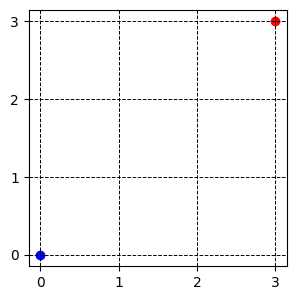
\includegraphics[width=0.3\textwidth]{figure/grid_grap.png}
    \caption{The grid graph of a simple IC routing problem.}
    \label{fig:grid}
\end{figure}

\subsection{GNN architectural design}
The GNN will utilize the message passing mechanism. It takes $\mathbf{X}$, $\mathbf{E}$, and $\mathbf{A}$ from the RL environment as input, and outputs the probability distribution of all the actions. The message network will be implemented by MLP, the messages will be aggregated by element-wise summation, and the node states will be updated by a gated recurrent unit (GRU). After the messaging passing stage, the node states will be feed into another MLP ended with a softmax layer to produce action probability distribution. 

Architecture of GNN can't reply on the graph topology. Like \#nodes. We want the GNN to generalize to graphs of any size. 

\subsection{RL policy training}
The proposed GNN will be embedded into our RL router as its policy network, which will be trained using PPO with RLlib. The parameters of the GNN will be updated by stochastic gradient descent, guided by the value feedback from the value network. 

%TODO: Briefly explain what is multi-agent RL and its advantages for our given problem. Also mention the paper which used a GNN as the policy network for the RL agent \cite{Almasan2022}. Also discuss the overall architecture of the GNN that we're going to use, and mention which libraries we're using (i.e., PyTorch, PyG, and RLLib). Adding a figure depicting the routing problem in a grid would also be very helpful. Also, don't forget to come up with a rough timeline and replace the 'X' values below!

\subsection{Project timeline}
\begin{itemize}
    \item Extended literature review (5 days)
    \item Designing the GNN prototype, combing with the RL router, and training on a simple benchmark (14 days)
    \item Testing the updated RL agent on benchmarks both similar to and different from the training benchmark (1 day)
    \item Analyzing the results and getting a measure of the generalizability (3 days)
    \item (bonus) Scaling up the model and design to support multi-agent concurrent routing (7 days)
    \item Writing the project report (14 days)
\end{itemize}
    
\section{Experiments}
We will implement a baseline MLP policy network, and train it with a simple benchmark.

\subsection{Comparing training efficiency}
In this experiment, we will train the GNN equipped router as well as the baseline router, both using a same benchmark. We will compare their plots of reward versus training iteration. The goal is to see how well the GNN equipped router trains comparing to the baseline. According to \cite{Wang2018}, we expect the new design will have similar or even better training efficiency.

\subsection{Comparing zero-shot performance} \label{m:0}
In this experiment, we will use the two zero-shot policies obtained during the previous experiment (one from the new design, one from the baseline) to run inference on several unseen benchmarks, which are netlists with canvas sizes, number of nets, and total number of pins per net similar to that of the training benchmark. We would then compare the results in terms of rewards, and solution qualities. We expect the new design would outperform the baseline.

\subsection{Comparing fine-tuning performance}
For this experiment, we will first run zero-shot inference on benchmarks with different number of nets, chip canvas size, and number of pins per net than the training benchmark. The goal is to see how well can the GNN scale to more complicated problems. We expect the zero-shot performance to be less sound than the results of the previous experiment, and hence, it is likely the policies need fine-tuning. We will fine-tune the polices for the same number of iterations, and compare the results in terms of rewards, and solution qualities. We expect the new design to do better than the baseline.

\begin{figure}[h!]
    \centering
    \begin{tikzpicture}
        \begin{axis}[
            axis lines = left,
            xlabel = Iteration,
            ylabel = Total loss,
            ymin=5, ymax=15,
            ]
            % The reward function
            \addplot [
            domain=0:100, 
            samples=100, 
            color=red,
            ]
            {10 + 2 * exp(-x / 20)};
            \addlegendentry{RL model}
            % Baseline
            \addplot [
            domain=0:100, 
            samples=100, 
            color=blue,
            ]
            {10};
            \addlegendentry{Baseline}
        \end{axis}
    \end{tikzpicture}
    \caption{Placeholder figure for total loss vs. time. Not related to any aforementioned experiments.}
\end{figure}

\begin{table}[h!]
    \caption{Placeholder table for the experiments. Not related to any aforementioned experiments.}
    \centering
    \begin{tabularx}{\textwidth}{LLLLLLL}
        \toprule
        \multicolumn{4}{c}{Benchmark specs} &
        \multicolumn{3}{c}{Results} \\
        \cmidrule(r){1-4}
        \cmidrule(r){5-7}
        Name & Canvas size & \# of nets & Avg. \# of pins per net & Runtime (s) & Max. memory usage (MB) & Total wirelength \\
        \midrule
        test1 & \(8 \times 8\) & 5 & 2.5 & 1.25 & 250 & 100 \\
        test2 & \(6 \times 6\) & 3 & 1 & 0.60 & 150 & 70 \\
        \bottomrule
    \end{tabularx}
\end{table}
    
%%%%%%%%%%%%%%%%%%%%%%%%%%%%%%%%%%%%%%%%%%%%%%%%%%%%%%%%%%%%
    
{
\small
\bibliographystyle{IEEEtranN}
\bibliography{references}
}

%%%%%%%%%%%%%%%%%%%%%%%%%%%%%%%%%%%%%%%%%%%%%%%%%%%%%%%%%%%%


\end{document}